\section{Základní nástroje statické analýzy}

\subsection{Debugger}
%% http://programujte.com/clanek/2006080803-cracking-2-cast/

Debugger je nástroj, který slouží primárně k ladění softwaru. Zároveň je ale také velmi důležitým nástrojem, pokud je potřeba zjistit, jak program pracuje. Umožňuje totiž krokovat kód instrukci po instrukci (v~případě interpretovaného kódu pak řádek po řádku) a zároveň sledovat změny hodnot v registrech, zásobníku nebo paměti.

Další důležitou funkcí debuggeru jsou breakpointy \cite{debugger_dissasembler}. Breakpoint lze nastavit kdekoliv v~kódu a jakmile na něj program narazí, vyvolá přerušeni. Je možné tedy například zjistit stav zásobníku v každém kroku smyčky.

Debuggerů existuje celá řada. Velmi populárním je například OllyDbg viz obrázek č. \ref{fig:olldbg}. Tento debugger umožňuje všechny potřebné funkce pro sledování registru, volání API, konstant, stringu atd. Má přívětivé uživatelské prostředí a lze do něj vložit externí rozšíření \cite{ollydbg}. Bohužel s ním lze debuggovat pouze 32-bitové aplikace.

\begin{figure}[!ht]
    \centering
    \caption{Debugger OllyDbg}
    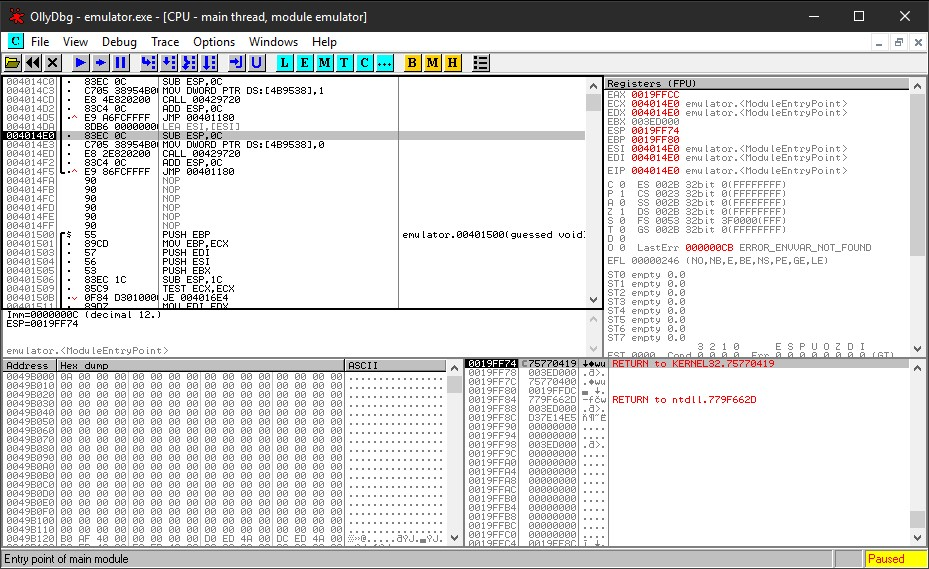
\includegraphics[width=140mm,scale=0.5]{Figures/obrazky/OllyDbg.jpg}
    \label{fig:olldbg}
\end{figure}

\subsection{Disassembler}
%what is that and how it works
%https://reverseengineering.stackexchange.com/questions/11466/how-does-disassembler-really-work

Disassembler umožňuje převod kódu zpět do programovacího jazyka nejčastěji assembleru \cite{debugger_dissasembler}. Existují také pokročilejší disassemblery, které umí převést strojový kód do C nebo jiného jazyka. Kvalita takovýchto převodů není valná (nezískáme původní zdrojový kód) a je vhodná spíše pro lepší orientaci v konstrukcích programu. Oproti debuggeru nelze dissasembleru v jeho procesu nijak zabránit. Proto však jsou využívány další techniky ochrany před analýzou jako obfuskace, komprese nebo šifrování.

%\paragraph*{Metoda lineárního průchodu}
%\paragraph*{Analýza rekurzivním sestupem}

\subsection{HEX editor}

HEX editor slouží ke zkoumání a editaci na úrovni bytů a bitů. Nejčastěji se souborem pracuje v šestnáctkové soustavě, proto tedy HEX editor. Některé editory také umožňuji zobrazit data jako ASCII nebo Unicode, hledat určité vzory apod. Existuje spousta HEX editorů. Vhodným  může být například \emph{FileInsight}, jehož autorem je společnost McAfee Labs. Tento editor je zachycen na obrázku č. \ref{fig:hexeditor}. Tento HEX editor zvládne kromě běžných funkcí, jako je například editace binárních dat, také zobrazit strukturu PE souboru, dissasemblovat 32-bitové aplikace nebo dekódovat některé metody obfuskace (XOR, posun, Base64) \cite{hexeditors}.

\begin{figure}[!ht]
    \centering
    \caption{HEX editor FileInsight}
    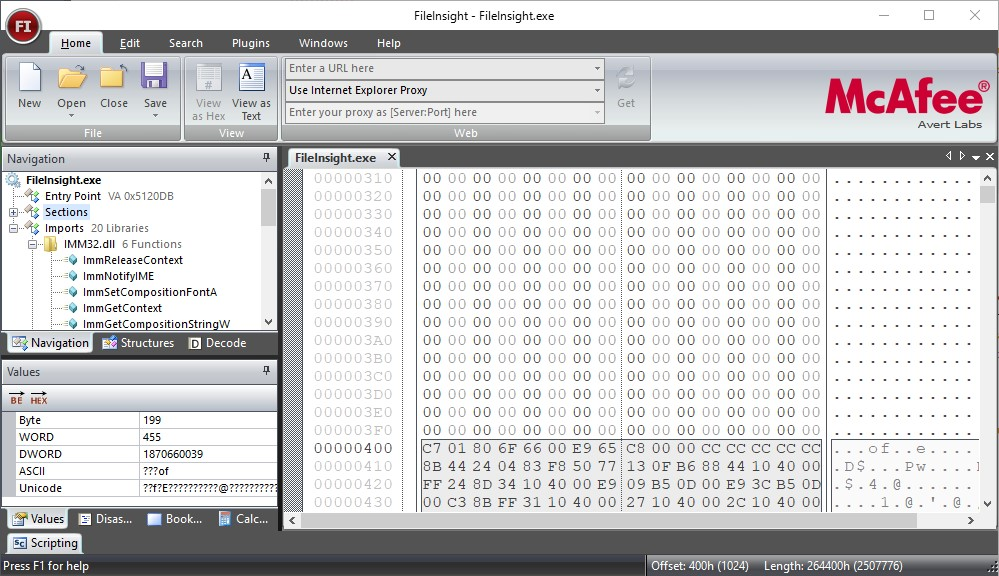
\includegraphics[width=150mm,scale=0.5]{Figures/obrazky/MCAfee-Insights.jpg}
    \label{fig:hexeditor}
\end{figure}

\subsection{Balík sysinternals}
%https://www.chip.cz/casopis-chip/01-2017/windows-sysinternals/
%https://docs.microsoft.com/en-us/sysinternals/

Balík programů sysinternals obsahuje nespočet utilit, které umožňují rozšířit základní funkce Windows \cite{chip_sysinternals}. Kolekce obsahuje například nástroje pro zjištění informací o systému, detailní správce běžících procesů apod. Tato sada je dostupná zdarma a lze stáhnout ze stránek Microsoftu.

Pro analýzu malwaru můžeme z této sady použít například aplikaci \emph{Strings} \cite{ms_sysinternals}, která slouží k extrakci obsažených řetězců v požadovaném souboru. V případě dynamické analýzy by bylo možné použít například \emph{Process Explorer}.

\subsection{Dependency Walker}
Tento nástroj slouží k analýze závislosti zkoumaného souboru. Umožňuje analyzovat různé moduly Windows (jako .exe, .dll, .ocx, .sys atd.) \cite{depedencywalker}. A to jak 32 bitové, tak 64 bitové. Následně jsou vazby zobrazeny programem v hierarchické stromové struktuře viz obrázek č. \ref{fig:depedency}. Dalším výstupem je seznam potřebných souborů včetně detailních informací o plné cestě k souboru atd.

\begin{figure}[!ht]
    \centering
    \caption{Dependency Walker}
    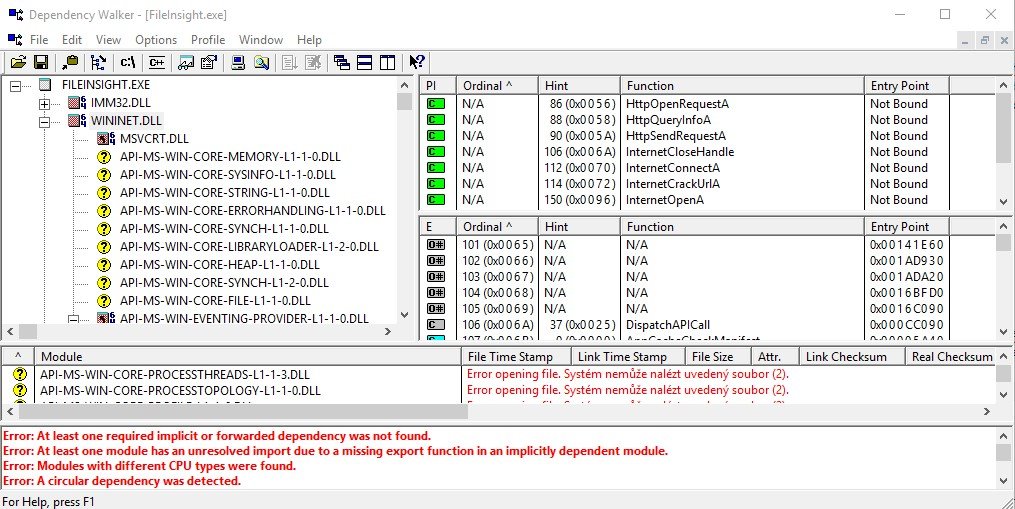
\includegraphics[width=150mm,scale=0.5]{Figures/obrazky/DependencyWalker.jpg}
    \label{fig:depedency}
\end{figure}
